

\section{Hashing}
Hash functions are a cryptographic primitive with many useful applications in computer science. Hashes are used to verify data integrity, and play an important role in entity authenticity and digital signature schemes. They can be used for cryptographic key derivation, key and pseudorandom number generation; moreover, blockchain principle is built entirely on hashing. Aforementioned applications are also prevalent in the context of lightweight cryptography \cite{lightHashTrends}. The following chapter is going to introduce a reader to hash functions in general and present the hashing design of the ASCON family.

% First, we will look at the theoretical requirements for the hash functions, and then proceed with the practical
\subsection{Hash function and its requirements}
Simply put, a cryptographic hash function $ \mX: \{0, 1\}^* \rightarrow \{0,1\}^{l} $ takes an input bitstring $x$ of arbitrary length and produces a short bitstring output $y$ of fixed length $l$, also called a digest, or a hash value. Such mapping allows us to identify any $x$ with some shorter $y$. 

\subsubsection{Collision resistance}
Theoretically, because the domain of possible inputs is larger than of the range of the hash function, and since the mapping is surjective, there is an infinite amount of possible messages, such that their hash values are identical. Since $ |\{0,1\}^*| $ is infinite and $ |\{0,1\}^l| = 2^l $, by the pigeonhole principle, there exist at least two bitstrings $ x_1, x_2 \in \{0,1\}^* $, with $ x_1 \neq x_2 $, such that $ \mX(x_1) = \mX(x_2) $. This equality of digests of two or more input values is called a collision.

Practically, it is very hard to find such collisions. The ``hardness'' is described by the theoretical amount of needed prompts to a hash function to acquire at least one of such events, and the requirement for a low probability of collision is called a \textit{collision resistance}. By simply trying out 
\[
\mX(x_1), \mX(x_2), \mX(x_3), \ldots
\]
and comparing each next hash value with previous ones, eventually, an attacker is going to stumble upon a collision. In order for $x_1, x_2, x_3, \ldots$ not to share a matching hash, each of these probed inputs must not yield a match with any other probed input. And since a number of possible hashes is finite, the probability of not having a single collision pair decreases exponentially with each new input. To find an expected amount of trials needed for a 50\% chance of getting a match, we can apply an approximation for the Birthday Problem: 
\[n\approx \sqrt{2d\cdot p}, \]
where $d$ is the number of possible outcomes, and $p$ is a desired probability. This yields us a $\sqrt{2^l} = 2^{l/2}$. For example, if a hash function produces a 256-bit digest, one has to probe $2^{128}$ number of inputs to merely have a 50\% chance of getting a pair of matching hashes, which is sufficiently infeasible under our current compute capabilities; moreover, one has to have a tremendous storage of at least $2^{133}$ bytes ($10^{25}$ petabytes) for such an endeavor.

\subsubsection{(Second-) preimage resistance}
If we would like to use hash functions as a reliable means to verify an integrity or authenticity of important information, two more requirements arise. One would not like, if an attacker, knowing the hash value $y$, easily guessed or picked a suitable input $\hat{x}$, such that $\mX(\hat{x}) = y$, because he could perfectly disguise the matching $\hat{x}$ as a valid piece of data, or worse, find out the true input. The property that allows to withstand such attacks is called \textit{one-wayness} or \textit{preimage resistance}, the $x$ being a preimage of $y$. The second undesirable situation is when an adversary can, for a given input $x$ that he knows, find such $x^\prime$ that $\mX(x^\prime) = \mX(x)$ and $x^\prime \neq x$. This means that we would like a hash function to ensure that it is hard to find not just any collision, but a specific one for a given input. This property is called a \textit{second-preimage resistance}. Both requirements yield a need to test $2^{l}$ number of inputs to break them, if a hash function is ideally constructed.

\subsubsection{Ideal hash function}
An ideal hash function is said to be following a \textit{random oracle model}, in which a random oracle samples and outputs hash values from a random uniform distribution each time a new input is fed. If a random oracle again receives an input that was given in the past, it yields the same hash as one he returned the first time for this input. The design of the hash functions is tested against the ideal random oracle model by theoretical proofs and is aimed to be sufficiently close to, or \textit{indifferentiable} from, it.

\subsection{Hash constructions}
The first widely used idea to bring an infinite domain to a finite range of hash values is to use a \textit{compression function} $f$. Message $M$ is first padded and split into chunks of equal length $M=x_1||x_2||x_3||\ldots||x_n$. A compression function then takes in a first input chunk with the initial state $S$. The previous output of the function and the next chunk of a message are then fed to the same function again, sequentially, until the message is fully expended. The end return is a hash value. This approach is called a \textit{Merkle-Damgård transform}. Its working is depicted schematically on the Figure \ref{fig:merkle}. SHA-1 and SHA-2 standard hashing algorithms were designed as Merkle-Damgård hash functions, the SHA-1 being now deprecated for discovered security flaws. In 2017, \cite{firstcollision} found the first ever collision for SHA-1.

\begin{figure}[H]
    \centering
        \tikzset{every picture/.style={line width=0.75pt}} %set default line width to 0.75pt        

        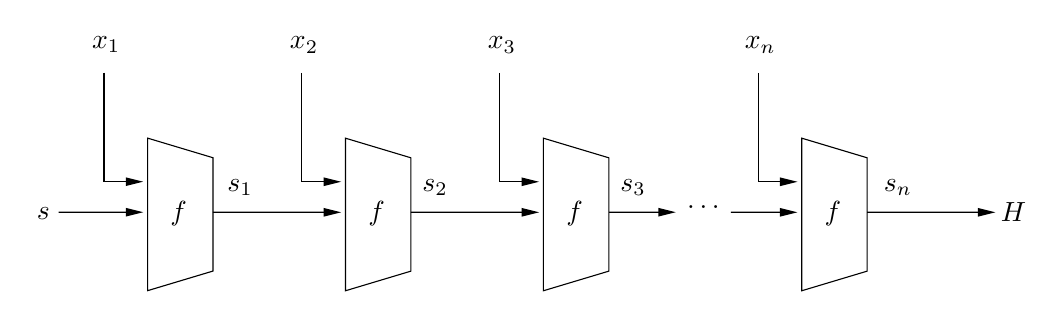
\begin{tikzpicture}[x=0.75pt,y=0.75pt,yscale=-1,xscale=1]
        %uncomment if require: \path (0,235); %set diagram left start at 0, and has height of 235
        
        %Shape: Trapezoid [id:dp989820392477355] 
        \draw   (82.75,62.7) -- (114.25,72.15) -- (114.25,126.76) -- (82.75,136.21) -- cycle ;
        
        %Straight Lines [id:da9136570431817581] 
        \draw    (39.9,98.4) -- (78.65,98.41) ;
        \draw [shift={(80.65,98.41)}, rotate = 180] [fill={rgb, 255:red, 0; green, 0; blue, 0 }  ][line width=0.08]  [draw opacity=0] (8.4,-2.1) -- (0,0) -- (8.4,2.1) -- cycle    ;
        %Straight Lines [id:da22262592186104624] 
        \draw    (61.75,31.19) -- (61.75,83.7) -- (78.65,83.7) ;
        \draw [shift={(80.65,83.7)}, rotate = 180] [fill={rgb, 255:red, 0; green, 0; blue, 0 }  ][line width=0.08]  [draw opacity=0] (8.4,-2.1) -- (0,0) -- (8.4,2.1) -- cycle    ;
        %Shape: Trapezoid [id:dp8730607411910694] 
        \draw   (178.11,62.74) -- (209.61,72.19) -- (209.61,126.8) -- (178.11,136.25) -- cycle ;
        
        %Straight Lines [id:da7073511289859868] 
        \draw    (114.25,98.44) -- (174,98.45) ;
        \draw [shift={(176,98.45)}, rotate = 180] [fill={rgb, 255:red, 0; green, 0; blue, 0 }  ][line width=0.08]  [draw opacity=0] (8.4,-2.1) -- (0,0) -- (8.4,2.1) -- cycle    ;
        %Straight Lines [id:da8571759413814846] 
        \draw    (157.1,31.23) -- (157.1,83.74) -- (174,83.74) ;
        \draw [shift={(176,83.74)}, rotate = 180] [fill={rgb, 255:red, 0; green, 0; blue, 0 }  ][line width=0.08]  [draw opacity=0] (8.4,-2.1) -- (0,0) -- (8.4,2.1) -- cycle    ;
        
        %Shape: Trapezoid [id:dp010143672535839032] 
        \draw   (273.46,62.74) -- (304.97,72.19) -- (304.97,126.8) -- (273.46,136.25) -- cycle ;
        
        %Straight Lines [id:da15113595456398543] 
        \draw    (209.61,98.44) -- (269.36,98.45) ;
        \draw [shift={(271.36,98.45)}, rotate = 180] [fill={rgb, 255:red, 0; green, 0; blue, 0 }  ][line width=0.08]  [draw opacity=0] (8.4,-2.1) -- (0,0) -- (8.4,2.1) -- cycle    ;
        %Straight Lines [id:da9161491017393608] 
        \draw    (252.46,31.23) -- (252.46,83.74) -- (269.36,83.74) ;
        \draw [shift={(271.36,83.74)}, rotate = 180] [fill={rgb, 255:red, 0; green, 0; blue, 0 }  ][line width=0.08]  [draw opacity=0] (8.4,-2.1) -- (0,0) -- (8.4,2.1) -- cycle    ;
        
        %Shape: Trapezoid [id:dp04826586579594827] 
        \draw   (397.94,62.74) -- (429.44,72.19) -- (429.44,126.8) -- (397.94,136.25) -- cycle ;
        
        %Straight Lines [id:da5983989156297147] 
        \draw    (363.81,98.44) -- (393.84,98.45) ;
        \draw [shift={(395.84,98.45)}, rotate = 180.01] [fill={rgb, 255:red, 0; green, 0; blue, 0 }  ][line width=0.08]  [draw opacity=0] (8.4,-2.1) -- (0,0) -- (8.4,2.1) -- cycle    ;
        %Straight Lines [id:da1340107169372431] 
        \draw    (376.93,31.23) -- (376.93,83.74) -- (393.84,83.74) ;
        \draw [shift={(395.84,83.74)}, rotate = 180] [fill={rgb, 255:red, 0; green, 0; blue, 0 }  ][line width=0.08]  [draw opacity=0] (8.4,-2.1) -- (0,0) -- (8.4,2.1) -- cycle    ;
        %Straight Lines [id:da7846820892857251] 
        \draw    (429.44,98.44) -- (489.19,98.45) ;
        \draw [shift={(491.19,98.45)}, rotate = 180] [fill={rgb, 255:red, 0; green, 0; blue, 0 }  ][line width=0.08]  [draw opacity=0] (8.4,-2.1) -- (0,0) -- (8.4,2.1) -- cycle    ;
        %Straight Lines [id:da02924524891297775] 
        \draw    (305.18,98.4) -- (335.21,98.41) ;
        \draw [shift={(337.21,98.41)}, rotate = 180.01] [fill={rgb, 255:red, 0; green, 0; blue, 0 }  ][line width=0.08]  [draw opacity=0] (8.4,-2.1) -- (0,0) -- (8.4,2.1) -- cycle    ;

        % Text Node
        \draw (92.5,91.85) node [anchor=north west][inner sep=0.75pt]    {$f$};
        % Text Node
        \draw (187.86,91.89) node [anchor=north west][inner sep=0.75pt]    {$f$};
        % Text Node
        \draw (158.15,17.85) node    {$x_{2}$};
        % Text Node
        \draw (253.51,17.85) node    {$x_{3}$};
        % Text Node
        \draw (283.21,91.89) node [anchor=north west][inner sep=0.75pt]    {$f$};
        % Text Node
        \draw (407.69,91.89) node [anchor=north west][inner sep=0.75pt]    {$f$};
        % Text Node
        \draw (32.55,99) node    {$s$};
        % Text Node
        \draw (377.98,17.85) node    {$x_{n}$};
        % Text Node
        \draw (350.54,96.0) node    {$\ldots$};
        % Text Node
        \draw (127.31,86.72) node    {$s_{1}$};
        % Text Node
        \draw (221.31,86.7) node    {$s_{2}$};
        % Text Node
        \draw (316.7,86.7) node    {$s_{3}$};
        % Text Node
        \draw (444.31,86.7) node    {$s_{n}$};
        % Text Node
        \draw (500,98.4) node    {$H$};
        % Text Node
        \draw (62.8,17.81) node    {$x_{1}$};
        \end{tikzpicture}
    \caption{The Merkle-Damgård construction.}
    \label{fig:merkle}
\end{figure}
In a Merkle-Damgård hash function, the \textit{internal state} is fully exposed, reflecting the hash of the input. If attacker knows the hash, he knows the final state of the compression function and can ``resume'' the calculation further with an appended message, producing a valid hash. This is known as a \textit{length extension attack} on hash.

A second architecture eliminates the length extension attack by never revealing the full internal state. This also conveniently allows for yielding an arbitrary length hash value. Such useful features are achieved by introducing a much larger internal state, allowing chunks of a message to be ``absorbed'' into the state, having a permutation function, and releasing a hash from the state also only chunk by chunk. This configuration is called a \textit{sponge construction}, and ASCON hashing adopts this particular mode of operation.

\begin{figure}[H]
    \centering
    \begin{tikzpicture}
        \SpongeInitInner{$\text{IV} \| 0^c\hskip-10pt$}{$p^a$}
        \draw (P.south) +(0,-1) node[spongephase] (phase) {Initialization\phantom{p}\qquad\null};
        \SpongeStep\SpongePhaseSep
    
        \SpongeAbsorb{$M_1$}{$p^b$}{$r$}{$c$}
        \SpongeEtc
        \SpongeAbsorb{$M_{s-1}$}{$p^b$}{$r$}{$c$}
        \draw (x|-phase) node[spongephase] {Absorb Message};
        \SpongeXorOuter{$M_s$}{$r$}{$c$}
        \SpongeStep\SpongePhaseSep\SpongeStep
        \SpongePermute{$p^a$}
    
        \SpongeSqueeze{$H_1$}{$p^b$}{$r$}{$c$}
        \SpongeEtc
        \SpongeSqueeze{$H_{\lceil \ell/r \rceil}$}{$p^b$}{$r$}{$c$}
        \draw (x|-phase) node[spongephase] {Squeeze Hash\qquad\null};
        \SpongeSkip
        \SpongeEtc
    \end{tikzpicture}
  \caption{The sponge construction of ASCON.}
%   \label{fig:sponge}
\end{figure}
A sponge function is made of three components: a state memory $S$ containing $b$ bits, a permutation function $p: \left\{0,1\right\}^b \rightarrow \left\{0,1\right\}^b$ and a padding function $P$:

\begin{itemize}
  \item $S$ is divided into two parts: the $r$-bit \textit{rate} $S_r$ and the $c$-bit \textit{capacity}~$S_c$. The rate is the part of the state that is XORed with the input message, while the capacity is the part that stays hidden. Both rate and capacity are then being permuted together by the function $p$;
  \item $p$ produces a pseudo random permutation of the $2^b$ possible states, details of which are shown in the next chapter about permutations;
  \item $P$ is a function that pads the input message to a multiple of $r$.
\end{itemize}

The sponge function is performed iteratively in two phases: the \textbf{absorbing phase} and the \textbf{squeezing phase}. During preprocessing, an input message is padded and cut into $r$ bit blocks $M_1||M_2||\ldots||M_s$. In the absorbing phase, blocks of the input message are mixed with $S_r$ using per bit XOR operation. Then a result is concatenated with the capacity and passed through $p$ to become a new state again:
\begin{equation}
    S \leftarrow p((S_r \oplus M_i)~||~S_c)~\text{for}~1 \leq i \leq s. \notag
\end{equation}


In the squeezing phase, the finalizing permutation is applied to $S$ and the first leftmost $r$ bits of the state are retrieved. This process is repeated until the outputs $H_1||H_2||\ldots||H_t$ reach the desired length $\ell$.

The last $c$ bits are neither XORed nor directly output. 